\documentclass[12pt,a4paper]{article}
\usepackage[margin=2.5cm]{geometry}
\usepackage{amsmath,amssymb}
\usepackage{listings}
\usepackage{xcolor}
\usepackage{tikz}
\usetikzlibrary{arrows.meta,automata,positioning,shapes.geometric,calc,fit,backgrounds}
\usepackage{booktabs}
\usepackage{hyperref}
\usepackage{enumitem}
\usepackage{fancyhdr}
\usepackage{titlesec}

\hypersetup{colorlinks=true,linkcolor=blue,urlcolor=blue}

\pagestyle{fancy}
\fancyhf{}
\rhead{PLC Lecture Notes}
\lhead{AIT MSCS Y1S2}
\cfoot{\thepage}

\lstdefinestyle{pascal}{
  language=Pascal,
  basicstyle=\small\ttfamily,
  keywordstyle=\bfseries,
  commentstyle=\itshape\color{gray},
  numbers=left,numberstyle=\tiny,
  frame=single,breaklines=true,
}
\lstdefinestyle{caml}{
  basicstyle=\small\ttfamily,
  keywordstyle=\bfseries\color{blue!70!black},
  frame=single,breaklines=true,
}
\lstdefinestyle{python}{
  language=Python,
  basicstyle=\small\ttfamily,
  keywordstyle=\bfseries\color{blue!70!black},
  commentstyle=\itshape\color{gray},
  frame=single,breaklines=true,
}

\title{\textbf{Programming Languages \& Compilers}\\[6pt]
\large Lecture Notes Summary\\[4pt]
\normalsize AIT Masters in Computer Science --- Year 1, Semester 2}
\author{Study Notes}
\date{2026}

\begin{document}
\maketitle
\tableofcontents
\newpage

% ============================================================
\section{Compiler Overview}
% ============================================================

A compiler translates source code through a sequence of well-defined phases.
Each phase transforms one representation into a lower-level, more machine-friendly one.

\begin{center}
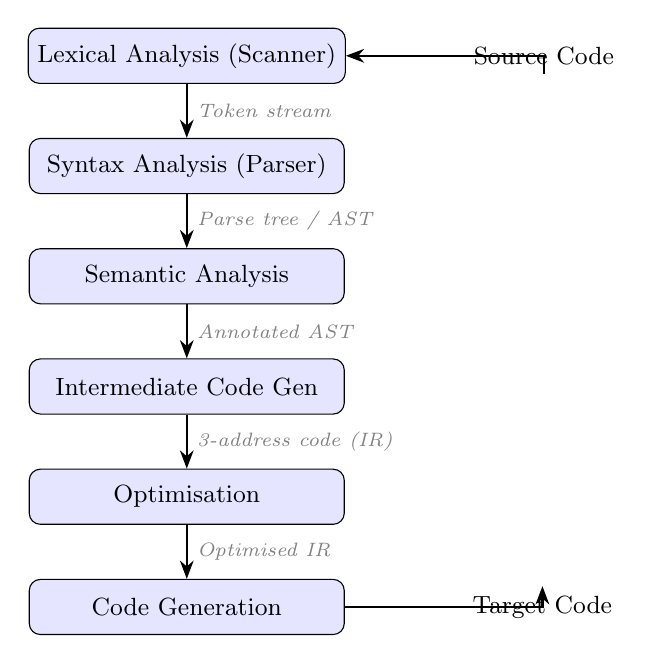
\begin{tikzpicture}[
  phase/.style={rectangle,draw,rounded corners=4pt,
                minimum width=4cm,minimum height=0.7cm,
                fill=blue!10,font=\small},
  arr/.style={-Stealth,thick},
  label/.style={font=\scriptsize\itshape,text=gray}
]
  \node[phase] (lex)   at (0,0)   {Lexical Analysis (Scanner)};
  \node[phase] (syn)   at (0,-1.4){Syntax Analysis (Parser)};
  \node[phase] (sem)   at (0,-2.8){Semantic Analysis};
  \node[phase] (ir)    at (0,-4.2){Intermediate Code Gen};
  \node[phase] (opt)   at (0,-5.6){Optimisation};
  \node[phase] (cg)    at (0,-7.0){Code Generation};

  \draw[arr] (lex) -- node[label,right]{Token stream} (syn);
  \draw[arr] (syn) -- node[label,right]{Parse tree / AST} (sem);
  \draw[arr] (sem) -- node[label,right]{Annotated AST} (ir);
  \draw[arr] (ir)  -- node[label,right]{3-address code (IR)} (opt);
  \draw[arr] (opt) -- node[label,right]{Optimised IR} (cg);

  \node[right=1.5cm of lex,font=\small] (src) {Source Code};
  \node[right=1.5cm of cg, font=\small] (tgt) {Target Code};
  \draw[arr] (src.south) |- (lex.east);
  \draw[arr] (cg.east)   -| (tgt.north);
\end{tikzpicture}
\end{center}

% ============================================================
\section{Lexical Analysis}
% ============================================================

The \textbf{scanner} reads the character stream and groups characters into
\emph{tokens} (terminal symbols of the grammar).

\begin{description}
  \item[Token] A pair $\langle\text{class}, \text{value}\rangle$,
        e.g.\ $\langle\mathtt{NUM}, 30\rangle$.
  \item[Lexeme] The actual character sequence matched, e.g.\ \texttt{"30"}.
  \item[Pattern] A regular expression describing valid lexemes for a token class.
\end{description}

\subsection{Tokens and Patterns}

\begin{center}
\begin{tabular}{lll}
\toprule
Token & Pattern (regex) & Example lexeme\\
\midrule
\texttt{NUM}   & $[\texttt{0-9}]^+$                 & \texttt{30}\\
\texttt{ID}    & $[\texttt{a-zA-Z\_}][\texttt{w}]^*$ & \texttt{count}\\
\texttt{PLUS}  & $\backslash\texttt{+}$              & \texttt{+}\\
\texttt{TIMES} & $\backslash\texttt{*}$              & \texttt{*}\\
\bottomrule
\end{tabular}
\end{center}

\subsection{DFA for \texttt{NUM} and \texttt{*}}

The scanner is implemented as a DFA.
Below is the combined DFA recognising \texttt{NUM} (one or more digits) and
\texttt{TIMES} (a single \texttt{*}).

\begin{center}
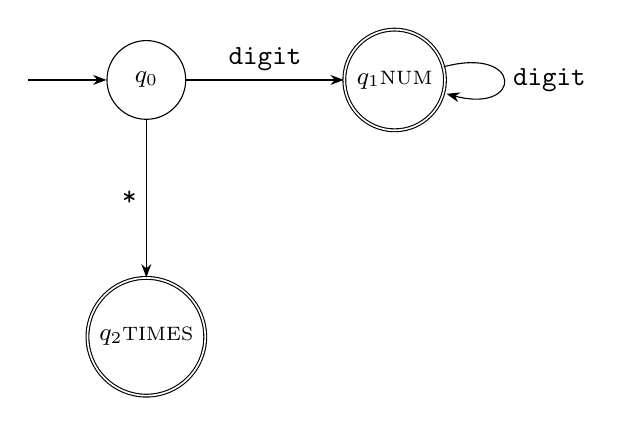
\begin{tikzpicture}[
  state/.style={circle,draw,minimum size=1cm,font=\small},
  acc/.style={circle,draw,double,minimum size=1cm,font=\small},
  arr/.style={-Stealth},
  >=Stealth
]
  \node[state]          (q0) {$q_0$};
  \node[acc,right=2cm of q0]  (q1) {$q_1$\\\scriptsize NUM};
  \node[acc,below=2cm of q0]  (q2) {$q_2$\\\scriptsize TIMES};

  \draw[arr] (-1.5,0) -- (q0);
  \draw[arr] (q0) -- node[above]{\texttt{digit}} (q1);
  \draw[arr] (q1) edge[loop right] node{\texttt{digit}} ();
  \draw[arr] (q0) -- node[left]{\texttt{*}} (q2);
\end{tikzpicture}
\end{center}

\subsection{Lexical Analysis Trace: \texttt{"30 * 4 \$"}}

\begin{center}
\begin{tabular}{llll}
\toprule
Input consumed & Token emitted & Class & Value\\
\midrule
\texttt{30} & $\langle\mathtt{NUM}, 30\rangle$ & NUM & 30\\
\texttt{*}  & $\langle\mathtt{TIMES}, \text{*}\rangle$ & TIMES & *\\
\texttt{4}  & $\langle\mathtt{NUM}, 4\rangle$  & NUM & 4\\
\texttt{\$} & end-of-input                    & ---  & ---\\
\bottomrule
\end{tabular}
\end{center}

\subsection{Pipeline: RegEx $\to$ NFA $\to$ DFA $\to$ Minimised DFA}

\begin{enumerate}
  \item Write a regular expression for each token class.
  \item Build an NFA via \emph{Thompson's construction}.
  \item Convert NFA $\to$ DFA via \emph{subset (powerset) construction}.
  \item Minimise the DFA via \emph{Hopcroft's algorithm}.
  \item Run the DFA on input; \emph{longest match} wins.
\end{enumerate}

% ============================================================
\section{Syntax Analysis (Parsing)}
% ============================================================

The \textbf{parser} checks that the token stream conforms to the grammar and
builds a parse tree or AST.

\subsection{Context-Free Grammars}

A CFG is a 4-tuple $G = (V, T, P, S)$ where $V$ is the set of non-terminals,
$T$ is the set of terminals, $P$ is the set of productions, and $S$ is the start symbol.

\textbf{Example grammar for arithmetic expressions:}
\begin{align*}
E &\to E + T \mid T \\
T &\to T * F \mid F \\
F &\to (E) \mid \mathbf{num}
\end{align*}

\subsection{Grammar Classification}

\begin{center}
\begin{tabular}{llll}
\toprule
Class & Strategy & Lookahead & Tool\\
\midrule
LL(1)           & Top-down, predictive & 1 token & Recursive descent\\
LR(0)           & Bottom-up, shift-reduce & 0 & Simplest SLR\\
SLR(1)          & Bottom-up, FOLLOW sets  & 1 & SLR\\
LALR(1)         & Bottom-up, lookahead    & 1 & yacc/bison (default)\\
Canonical LR(1) & Full LR, largest tables & 1 & Most powerful\\
\bottomrule
\end{tabular}
\end{center}

\subsection{LL(1) Parsing}

\begin{description}
  \item[\textbf{FIRST}($\alpha$)] Set of terminals that can begin strings derived from $\alpha$.
  \item[\textbf{FOLLOW}(A)] Set of terminals that can appear immediately after $A$.
\end{description}

Parse table entry:
\[
M[A,\,a] = A \to \alpha \quad \text{if } a \in \text{FIRST}(\alpha),
\qquad
M[A,\,a] = A \to \alpha \quad \text{if } \varepsilon \in \text{FIRST}(\alpha) \text{ and } a \in \text{FOLLOW}(A).
\]

\subsection{Shift-Reduce (LR) Parsing}

The parser maintains a \emph{stack} and inspects the remaining \emph{input}:
\begin{description}
  \item[Shift] Push the next input token onto the stack.
  \item[Reduce] Pop the \emph{handle} $\beta$ from the stack; push LHS non-terminal $A$
        (for production $A \to \beta$).
  \item[Accept] Input fully consumed and stack contains only the start symbol.
  \item[Error] No valid action.
\end{description}

\textbf{Conflicts:}
\begin{itemize}
  \item \emph{Shift-Reduce conflict}: ambiguous whether to shift the next token or reduce.
  \item \emph{Reduce-Reduce conflict}: two productions can reduce the same handle.
\end{itemize}

\subsubsection{LR(0) Items and Closure}

An \textbf{LR(0) item} is a production with a dot marking parse progress:
\[
E \to E + \bullet\, T \quad (\text{expecting } T \text{ next})
\qquad
E \to E + T\, \bullet \quad (\text{ready to reduce})
\]

\textbf{Closure}$(I)$: for every item $[A \to \alpha \bullet B \beta]$ in $I$,
add all items $[B \to \bullet\, \gamma]$.

\textbf{Goto}$(I, X)$: move the dot past $X$ in every applicable item of $I$.

\subsection{Parse Tree Example: \texttt{n + n * n}}

\begin{center}
\begin{tikzpicture}[
  every node/.style={font=\small},
  level 1/.style={sibling distance=5cm},
  level 2/.style={sibling distance=3cm},
  level 3/.style={sibling distance=2cm},
  edge from parent/.style={draw,-}
]
\node {$E$}
  child { node {$E$}
    child { node {$T$}
      child { node {$F$}
        child { node {\texttt{n}} }
      }
    }
  }
  child { node {\texttt{+}} }
  child { node {$T$}
    child { node {$T$}
      child { node {$F$}
        child { node {\texttt{n}} }
      }
    }
    child { node {\texttt{*}} }
    child { node {$F$}
      child { node {\texttt{n}} }
    }
  };
\end{tikzpicture}
\end{center}

% ============================================================
\section{The AIT Acceptor (PDA-based LR Parser)}
% ============================================================

For languages that require $\text{LR}(n > 1)$ lookahead, the course introduces
the \textbf{AIT acceptor}, a pushdown automaton tailored to shift-reduce parsing.

\subsection{Definition}

An AIT acceptor is a \textbf{sextuple}
\[
M = (K,\, \Sigma,\, \Gamma,\, \Delta,\, s,\, F)
\]
where
\begin{description}[leftmargin=2cm]
  \item[$K$] Finite set of states.
  \item[$\Sigma$] Input alphabet.
  \item[$\Gamma$] Stack alphabet.
  \item[$\Delta$] Set of transitions
        $(q,\, a,\, \beta) \to (q',\, \gamma,\, i)$
        where $i \in \{0, 1\}$:\\
        $i=1$ consume input symbol; $i=0$ do not consume input.
  \item[$s$] Start state.
  \item[$F$] Set of accepting states.
\end{description}

\subsection{Configurations}

A \textbf{configuration} is a triple $(q,\, w,\, v)$:
\begin{itemize}
  \item $q \in K$ --- current state.
  \item $w \in \Sigma^*$ --- remaining input.
  \item $v \in \Gamma^*$ --- current stack contents (top at left).
\end{itemize}

\textbf{Initial configuration}: $(s,\, w_0,\, \varepsilon)$.

\textbf{Acceptance}: $(q_f,\, \varepsilon,\, \varepsilon)$ for some $q_f \in F$.

\subsection{Example: Balanced Parentheses}

Grammar: $S \to (S) \mid SS \mid \varepsilon$.
Step-by-step trace on input \texttt{(())}:

\begin{center}
\begin{tabular}{llll}
\toprule
State & Input remaining & Stack & Action\\
\midrule
$q_0$ & \texttt{(())} & $\varepsilon$ & Shift \texttt{(}\\
$q_0$ & \texttt{())}  & \texttt{(}    & Shift \texttt{(}\\
$q_0$ & \texttt{))}   & \texttt{((}   & Shift \texttt{)}\\
$q_0$ & \texttt{)}    & \texttt{(}    & Reduce $S \to (S)$\\
$q_0$ & \texttt{)}    & $S$           & Shift \texttt{)}\\
$q_0$ & $\varepsilon$ & $S$           & Reduce $S \to (S)$\\
$q_f$ & $\varepsilon$ & $\varepsilon$ & \textbf{Accept}\\
\bottomrule
\end{tabular}
\end{center}

\begin{center}
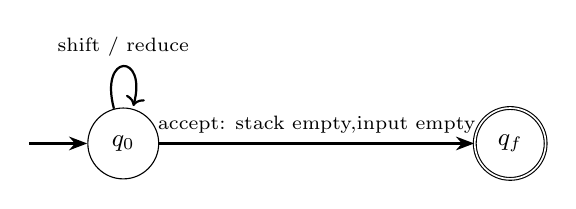
\begin{tikzpicture}[
  state/.style={circle,draw,minimum size=0.9cm,font=\small},
  acc/.style={circle,draw,double,minimum size=0.9cm,font=\small},
  arr/.style={-Stealth,thick}
]
  \node[state]         (q0) {$q_0$};
  \node[acc,right=4cm of q0] (qf) {$q_f$};
  \draw[arr] (-1.2,0) -- (q0);
  \draw[arr] (q0) edge[loop above] node[font=\scriptsize]{shift / reduce} ();
  \draw[arr] (q0) -- node[above,font=\scriptsize]{accept: stack empty,\\input empty} (qf);
\end{tikzpicture}
\end{center}

% ============================================================
\section{Values and Types}
% ============================================================

A \textbf{value} is anything that can be evaluated, stored, incorporated in a data
structure, passed as an argument, or returned as a function result.

Values are grouped into \textbf{types} — sets of values sharing characteristic operations.
Types may be \emph{primitive}, \emph{composite}, or \emph{recursive}.

\subsection{Primitive Types of Pascal}

\begin{description}
  \item[Integer] Range $-32768 \ldots 32767$.
        Operations: $+,-,\times,\div,\mathbf{mod}$; conversion to real.
        Relations: $<,\leq,>,\geq,=$.
  \item[Real] Single and double precision.
  \item[Char] ASCII characters. Operations: \textit{Ord}, \textit{Chr}, \textit{Pred}, \textit{Succ}.
  \item[Boolean] Values: \textit{True}, \textit{False}.
        Logical: \textit{not}, \textit{and}, \textit{or}.
        Ordinal: \textit{Ord}(False)$=0$, \textit{Ord}(True)$=1$.
  \item[Enumerated] User-defined ordinal type.
        \texttt{type Day = (Sunday, Monday, \ldots, Saturday);}
  \item[Subrange] Subset of an ordinal host type.
        \texttt{type Lowercase = 'a'..'z';}
\end{description}

\subsection{Composite Types of Pascal}

Composite types are built via set-theoretic operations:
Cartesian products, disjoint unions, powersets, and function (mapping) types.

\subsubsection{Record (Cartesian Product)}

\begin{lstlisting}[style=pascal,numbers=none]
type Employee = record
                  Age    : Integer;
                  Gender : Char;
                end;
\end{lstlisting}
Values are $n$-tuples: $\text{Integer} \times \text{Char}$.

\subsubsection{Variant Record (Disjoint Union)}

\begin{lstlisting}[style=pascal,numbers=none]
type Accuracy = (exact, appro);
     Number   = record
                  case acc : Accuracy of
                    exact : (ival: Integer);
                    appro : (rval: Real);
                  end;
\end{lstlisting}
The tag field \textit{acc} determines which variant is active.

\subsubsection{Set (Powerset)}

\begin{lstlisting}[style=pascal,numbers=none]
type settype = set of basetype;   { basetype must be ordinal }
\end{lstlisting}
Operations: $\in$ (\textbf{in}), union ($+$), intersection ($*$), difference ($-$).

\subsubsection{Array (Function Type)}

\begin{lstlisting}[style=pascal,numbers=none]
type arraytype = array[subscripttype] of elementtype;
\end{lstlisting}
Values are functions $\text{subscripttype} \to \text{elementtype}$.
The subscript type must be a finite ordinal type.

\subsection{Types in Camllight}

\begin{description}
  \item[Integer] Range $-2^{30} \ldots 2^{30}-1$, arithmetic wraps modulo $2^{31}$.
        No operator overloading; integer and float operators are distinct.
  \item[Float] Separate operators: \texttt{+.}, \texttt{-.}, \texttt{*.}, \texttt{/.},
        \texttt{sqrt}, trig functions, \texttt{int\_of\_float}/\texttt{float\_of\_int}.
  \item[Product types (tuples)] \texttt{t * t'} defined automatically.
        Constructor \texttt{(,)}; projection \texttt{fst}/\texttt{snd}.
  \item[Generic abstraction] Parameterised over types:
        \texttt{\#type ('a,'b) pair = \{Fst: 'a; Snd: 'b\};;}
\end{description}

% ============================================================
\section{Type Checking}
% ============================================================

A \textbf{type system} assigns types to expressions and enforces type safety.

\subsection{Static vs.\ Dynamic Typing}

\begin{description}
  \item[Static typing] Types checked at compile time.
        Languages: Pascal, Java, ML, Camllight.
        Catches type errors before execution.
  \item[Dynamic typing] Types checked at runtime.
        Languages: Lisp, Smalltalk.
        More flexible but errors only discovered at execution.
\end{description}

\textbf{Rule:} Languages with static typing adopt \emph{static binding};
languages with dynamic typing adopt \emph{dynamic binding}.
Mixing static typing with dynamic binding breaks the static type checker.

\subsection{Type Expressions (Simple Language)}

Type expressions for Simple Language 1:
\[
\tau ::= \mathbf{int} \mid \mathbf{real} \mid \mathbf{bool}
\]

\subsection{Type Checking Rules}

The function \texttt{addtype(id, type)} inserts a new type binding into the symbol table.
The function \texttt{lookup(id)} retrieves the type.

\textbf{Inference rule for addition:}
\[
\frac{\Gamma \vdash e_1 : \mathbf{int} \quad \Gamma \vdash e_2 : \mathbf{int}}
     {\Gamma \vdash e_1 + e_2 : \mathbf{int}}
     \quad\text{(T-Plus)}
\]

\subsection{Type Equivalence}

\begin{description}
  \item[Name equivalence] Two types are equal iff they have the \emph{same name}.
        Used in Pascal for record types.
  \item[Structural equivalence] Two types are equal iff they have the \emph{same structure}.
        Used for arrays and pointers in Pascal.
\end{description}

% ============================================================
\section{Syntax-Directed Translation (SDT)}
% ============================================================

In SDT each grammar symbol carries one or more \textbf{attributes}.
Semantic rules attached to productions define how attribute values are computed.

\subsection{Attribute Types}

\begin{description}
  \item[Synthesised] Computed \emph{bottom-up} from children.
  \item[Inherited] Passed \emph{top-down} from parent or siblings.
\end{description}

\subsection{Ambiguity and Associativity}

The grammar $E \to E - E \mid \mathbf{num}$ is ambiguous.
Ambiguity affects evaluation order:
\begin{itemize}
  \item Left-associative: $10 - 5 - 2 = (10-5)-2 = 3$.
  \item Right-associative: $10 - 5 - 2 = 10-(5-2) = 7$.
\end{itemize}

Unambiguous left-recursive grammar: $E \to E - T \mid T$, \;$T \to \mathbf{num}$.

\subsection{Prefix and Postfix Notation}

For the expression $10 - 5 - 2$ (left-associative):
\begin{itemize}
  \item \textbf{Prefix:} \texttt{- - 10 5 2}
  \item \textbf{Infix:}  \texttt{10 - 5 - 2}
  \item \textbf{Postfix:} \texttt{10 5 - 2 -}
\end{itemize}

The \textbf{prefix attribute} $E.\textit{prf}$ is a synthesised attribute built bottom-up:
\[
E \to E_1 - T \qquad E.\textit{prf} := \texttt{"-"} \mathbin{\|} E_1.\textit{prf} \mathbin{\|} T.\textit{prf}
\]

\subsection{Appendix: Recursive Top-Down Parser-Translator}

A translation scheme embeds semantic actions within grammar productions.
The scheme can be executed directly as a recursive descent parser-translator.

\textbf{Example grammar with embedded actions:}
\begin{align*}
E  &\to T\; R\\
R  &\to \mathbf{addop}\; T\; \{\textit{print}(\mathbf{addop}.\textit{lexeme})\}\; R_1 \mid \varepsilon\\
T  &\to \mathbf{num}\; \{\textit{print}(\mathbf{num}.\textit{lexeme})\}
\end{align*}

A left-recursive SDT grammar with synthesised attribute $E.\mathit{val}$:
\[
E \to E_1 + \mathbf{num} \;\{E.\mathit{val} := E_1.\mathit{val} + \mathbf{num}.\mathit{lex}\}
\]
is transformed by eliminating left recursion, introducing inherited attribute $E'.\mathit{i}$
and output attribute $E'.\mathit{o}$, then converted to a recursive top-down translator.

% ============================================================
\section{Intermediate Code Generation (Three-Address Code)}
% ============================================================

\textbf{Three-address code} (3AC) has at most one operator per statement.

\subsection{Five Forms of 3AC Statements}

\begin{enumerate}
  \item $x := y \;\mathbf{op}\; z$ \quad (binary operation)
  \item $x := \mathbf{op}\; y$ \quad (unary operation)
  \item $x := y$ \quad (copy)
  \item $\mathbf{goto}\; L$ \quad (unconditional jump)
  \item $\mathbf{if}\; x \;\mathit{relop}\; y\; \mathbf{goto}\; L$ \quad (conditional jump)
\end{enumerate}

\subsection{Syntax-Directed Code Generation}

Each non-terminal $E$ carries two attributes:
\begin{description}
  \item[$E.\textit{place}$] The name of the variable or temporary holding the value.
  \item[$E.\textit{code}$] The sequence of 3AC statements to compute the value.
\end{description}

The function \texttt{new\_var()} generates a fresh temporary variable name.

\textbf{Semantic rules for Simple Language (key rules):}

\begin{center}
\begin{tabular}{ll}
\toprule
Production & Semantic rule\\
\midrule
$A \to \mathbf{id} := E$
  & $A.\textit{code} = E.\textit{code} \mathbin{\|} \mathbf{id}.\mathit{place} := E.\mathit{place}$\\
$E \to E_1 + E_2$
  & $E.\textit{place} = \texttt{new\_var()}$\\
  & $E.\textit{code} = E_1.\textit{code} \mathbin{\|} E_2.\textit{code} \mathbin{\|} E.\mathit{place} := E_1.\mathit{place} + E_2.\mathit{place}$\\
$E \to \mathbf{num}$
  & $E.\textit{place} = \mathbf{num}.\textit{val};\quad E.\textit{code} = \varepsilon$\\
$E \to \mathbf{id}$
  & $E.\textit{place} = \mathbf{id}.\textit{name};\quad E.\textit{code} = \varepsilon$\\
\bottomrule
\end{tabular}
\end{center}

\subsection{Annotated Parse Tree Example: \texttt{x = x + y + 2}}

\begin{center}
\begin{tikzpicture}[
  every node/.style={font=\small},
  level 1/.style={sibling distance=7cm},
  level 2/.style={sibling distance=4cm},
  level 3/.style={sibling distance=2.5cm},
  edge from parent/.style={draw,-}
]
\node {$A$: \textit{code}=[\texttt{nv0=x+y; nv1=nv0+2; x=nv1}]}
  child { node {\texttt{x}} }
  child { node {\texttt{:=}} }
  child { node {$E$: \textit{place}=\texttt{nv1}}
    child { node {$E$: \textit{place}=\texttt{nv0}}
      child { node {$E$: \textit{place}=\texttt{x}} child { node {\texttt{x}} } }
      child { node {\texttt{+}} }
      child { node {$E$: \textit{place}=\texttt{y}} child { node {\texttt{y}} } }
    }
    child { node {\texttt{+}} }
    child { node {$E$: \textit{place}=\texttt{2}} child { node {\texttt{2}} } }
  };
\end{tikzpicture}
\end{center}

Generated 3AC:
\begin{verbatim}
nv0 := x + y
nv1 := nv0 + 2
x   := nv1
\end{verbatim}

% ============================================================
\section{Storage and Variables}
% ============================================================

\subsection{The Store Model}

A \textbf{store} is a collection of \emph{cells} (locations).
Each cell is either \emph{allocated} or \emph{unallocated}.
An allocated cell contains either a \emph{storable value} or is \emph{undefined}.

\textbf{Variable declaration in Pascal:}
\texttt{var n: Integer} has two effects:
(1) an unallocated cell is found and \emph{bound} to $n$;
(2) its status becomes allocated with content \emph{undefined}.

At the end of the block containing the declaration, the cell reverts to unallocated.

\subsection{Storable Values}

\textbf{Storable values} are values that can be stored in a single cell.

\begin{center}
\begin{tabular}{ll}
\toprule
Language & Storable values\\
\midrule
Pascal & Primitive values, sets, pointers\\
Java   & All primitive values and object references (arrays are objects)\\
\bottomrule
\end{tabular}
\end{center}

The design of what is storable profoundly affects language compactness.

\subsection{Composite Variables}

A composite variable is a collection of variables whose contents form the
components of a composite value.
\begin{lstlisting}[style=pascal,numbers=none]
type Employee = record Age: Integer; Gender: Char; end;
var Peter, Copy: Employee;
Peter.Age := 21;  Peter.Gender := 'M';
Copy := Peter;    { shorthand for: Copy.Age:=Peter.Age; Copy.Gender:=Peter.Gender }
\end{lstlisting}

\textbf{Pascal vs.\ Java arrays:}
\begin{itemize}
  \item \textbf{Pascal}: \texttt{Y := X} copies the array value (value semantics).
        After \texttt{Y[0] := 5}, \texttt{X[0]} remains 1.
  \item \textbf{Java}: \texttt{int[] Y = X} copies the \emph{reference}.
        After \texttt{Y[0] = 5}, \texttt{X[0]} is also 5 (alias).
\end{itemize}

\subsection{Lifetime of Variables}

The \textbf{lifetime} of a variable is the interval between its creation and deletion.

\begin{description}
  \item[Local variable] Created for use only within a block; destroyed at block exit.
  \item[Global variable] Created in the outermost block; lives for the entire program.
\end{description}

\subsection{Dangling References}

A \textbf{dangling reference} occurs when a pointer refers to a cell that has been
deallocated (via \textbf{dispose} in Pascal).

\begin{lstlisting}[style=pascal,numbers=none]
new(X);  new(Y);  X^ := 2;  Y^ := X;  Writeln(Y^^);
dispose(X);   { cell X pointed to is freed }
new(Z);  Z := 4;
Writeln(Y^^); { DANGER: Y still points to the freed cell, now reused by Z }
\end{lstlisting}

Java avoids dangling references by preventing explicit deallocation; a
\emph{Garbage Collector} automatically disposes unreachable objects.

\subsection{Commands}

\textbf{Commands} update the store.
Basic kinds: \emph{skip}, \emph{assignment}, \emph{procedure calls},
\emph{sequential}, \emph{iterative}, \emph{expressions with side-effects}.

% ============================================================
\section{Bindings and Environments}
% ============================================================

\subsection{Bindings and Environments}

A \textbf{binding} associates an identifier with an entity; it is produced by a
\emph{declaration}.

An \textbf{environment} is a set of bindings where each identifier is bound to at most one entity.

\textbf{Example --- Pascal program environment at two points:}

At point (1) (main body): $\{c \mapsto \text{cell}_{\text{char}},\; q \mapsto \text{proc-abstraction},\; z \mapsto 0\}$.

At point (2) (inside procedure $Q$): $\{b \mapsto \text{cell}_{\text{bool}},\; c \mapsto 2.5,\; q \mapsto \text{proc-abstraction},\; z \mapsto 0\}$.

\subsection{Bindable Entities}

\begin{center}
\begin{tabular}{lp{7cm}}
\toprule
Language & Bindable entities\\
\midrule
Pascal      & Primitive values, strings, locations, procedure/function abstractions, types.
              \newline\textit{Note:} Composite values (records, sets, arrays) are \emph{not} bindable.\\
Camllight   & Primitive values, composite values, procedure/function abstractions, types, exceptions.\\
Java        & Primitive values, objects, locations, object methods, classes, interfaces, exceptions.\\
\bottomrule
\end{tabular}
\end{center}

\subsection{Scope}

Each declaration has a \textbf{scope} — the block in which it is visible.

\begin{description}
  \item[Binding occurrence] Where the identifier is declared (\texttt{var x: Integer}).
  \item[Applied occurrence] Where the identifier is used (\texttt{y := x + 1}).
\end{description}

If the same identifier is declared in two nested blocks, the inner declaration
\emph{shadows} (hides) the outer one.

\subsection{Static vs.\ Dynamic Binding}

\begin{description}
  \item[Static binding] The body of a function/procedure abstraction is evaluated in
        the \emph{environment of its definition} (lexical scope).
        Used by Pascal, ML, Java.
  \item[Dynamic binding] The body is evaluated in the \emph{environment of the call site}.
        Used by Lisp, Smalltalk.
\end{description}

\textbf{Key interaction:} Static typing + dynamic binding is problematic.
Under dynamic binding, type correctness of a function call depends on which
binding of free variables is in scope at call time — this can only be checked at runtime,
defeating the purpose of a static type checker.

\textbf{Dynamic binding example in Clisp:}
\begin{lstlisting}[style=caml,numbers=none]
> (defvar s 2)
> (defun f(d) (* d s))
> (defun g() (let ((s 3)) (f 3)))  ; rebinds s to 3 locally
> (f 3)  ; => 6  (uses s=2)
> (g)    ; => 9  (dynamic: f sees s=3 from g's environment)
\end{lstlisting}

\subsection{Declarations and Blocks}

\begin{description}
  \item[Block commands] A command containing a declaration whose bindings are used
        only for that command.
  \item[Block expressions] An expression containing a declaration whose bindings
        are used only for that expression.
  \item[Block declarations] A declaration containing local declarations whose bindings
        are used only for elaborating that declaration.
\end{description}

\textbf{The Qualification Principle:} Blocks are allowed for expressions, commands,
and declarations. This principle is the cornerstone of information hiding (encapsulation).
Java realises it through \texttt{class} with \texttt{public}/\texttt{private} modifiers.

% ============================================================
\section{Abstraction}
% ============================================================

\textbf{Abstraction} distinguishes \emph{what} a program does from \emph{how} it is
implemented.

\subsection{Function Abstraction}

A \textbf{function abstraction} abstracts over an expression; when called, it returns
a value.

\textbf{Camllight:}
\begin{lstlisting}[style=caml,numbers=none]
# let rec power = function x, n ->
    if n = 1 then x else x * power(x, n-1);;
\end{lstlisting}

\textbf{Pascal:}
\begin{lstlisting}[style=pascal,numbers=none]
function power(x: Integer; n: Integer): Integer;
begin
  if n = 1 then power := x
  else power := x * power(x, n-1)
end;
\end{lstlisting}

\textbf{Note:} In Pascal, the identifier \texttt{power} denotes both a variable
(for returning the result) and the function abstraction in the same scope,
which can cause confusion.

\subsection{Procedure Abstraction}

A \textbf{procedure abstraction} abstracts over a \emph{command} for updating variables.
The caller observes only the effects of updating variables, not the execution details.

\subsection{Generic Abstraction}

\textbf{Generic abstraction} parameterises over types.
Pascal requires fixed types for parameters; Camllight supports polymorphism:
\begin{lstlisting}[style=caml,numbers=none]
# type ('a, 'b) pair = {Fst: 'a; Snd: 'b};;
\end{lstlisting}

\subsection{Parameter Mechanisms}

When an abstraction is called, actual parameters are passed to formal parameters.

\subsubsection{Copying Mechanism}

\begin{description}
  \item[Value parameter] A local variable is created and assigned the argument value on entry.
  \item[Result parameter] A local variable is created; on exit its value is assigned back
        to the argument variable.
  \item[Value-Result parameter] Combination: copy in on entry, copy out on exit.
\end{description}

\subsubsection{Definitional Mechanism}

\begin{description}
  \item[Constant parameter] Formal parameter is bound directly to the argument value.
  \item[Variable parameter (\texttt{var})] Formal parameter is bound to the argument
        variable (i.e.\ the \emph{location}, not the value).
        \textbf{Aliasing risk:} \texttt{confuse(i, i)} with \texttt{var m, n} makes
        $m$ and $n$ aliases for the same cell.
  \item[Function/Procedure parameter] Formal parameter is bound to a function/procedure abstraction.
\end{description}

Camllight uses definitional mechanism only.
Pascal uses both value parameters and variable (\texttt{var}) parameters.

\subsection{The Correspondence Principle}

\textit{For each form of declaration there is a corresponding form of parameter
mechanism, and vice versa.}

Camllight satisfies this principle (variable parameter $\leftrightarrow$ \texttt{let s = r;;}).
Pascal \emph{does not}: there is no declaration with the same effect as Pascal's
\texttt{var} parameter.

\subsection{Evaluation Order}

\begin{description}
  \item[Eager evaluation] Actual parameters are evaluated \emph{once} before the
        abstraction body executes.
        $\text{sqr}(p+q)$ with $p=2,q=5$: evaluate $p+q=7$ first, then $7*7=49$.
  \item[Normal evaluation] Formal parameter is bound to the \emph{unevaluated expression};
        evaluated each time it is needed.
        $\text{sqr}(p+q)$: compute $(2+5)*(2+5)=49$.
\end{description}

For pure functional programs (no side effects), both strategies yield the same result
(\textbf{Church-Rosser Property}):
\textit{If an expression can be evaluated at all, normal-order evaluation will find the
result; all terminating strategies yield the same value.}

For expressions with side effects (Pascal, Camllight), evaluation order matters:

\begin{lstlisting}[style=caml,numbers=none]
# let x = ref 1;;
# let f = function () -> x := !x + 1; !x;;
# f() + !x;;    (* evaluates right-to-left in Camllight: 3 *)
# !x + f();;    (* evaluates right-to-left: 4 *)
\end{lstlisting}

Camllight uses \textbf{eager (right-to-left) evaluation}.

% ============================================================
\section{Summary Table}
% ============================================================

\begin{center}
\begin{tabular}{lccc}
\toprule
Feature & Pascal & Camllight & Java\\
\midrule
Typing & Static & Static & Static\\
Binding & Static & Static & Static\\
Storable composites & No & Yes (tuples) & Yes (objects)\\
Generic abstraction & No & Yes & Yes (generics)\\
Parameter mechanism & Value + Var & Definitional & Value (refs for objects)\\
Garbage collection & No & Yes & Yes\\
Correspondence principle & No & Yes & Partial\\
Evaluation order & Left-to-right & Right-to-left & Left-to-right\\
\bottomrule
\end{tabular}
\end{center}

\end{document}
